\chapter{Ingegneria dei requisiti}
\begin{redbar}
I requisiti per un sistema sono le descrizioni dei servizi che un sistema dovrebbe fornire e i vincoli relativi al suo funzionamento. Il processo di scoperta, analisi, documentazione e verifica di questi servizi e vincoli è chiamato \textbf{ingegneria dei requisiti} (RE).
\end{redbar}

Il termine "requisito" non è utilizzato in modo uniforme nell'industria del software. In alcuni casi, un requisito è semplicemente una dichiarazione astratta di alto livello di un servizio che un sistema dovrebbe fornire o di un vincolo sul sistema. All'estremo opposto, è una definizione formale e dettagliata di una funzione del sistema.

\begin{center}
\begin{minipage}{0.9\textwidth}
\textit{Se un'azienda desidera stipulare un contratto per un grande progetto di sviluppo software, deve definire le proprie esigenze in modo sufficientemente astratto affinché la soluzione non sia predefinita. I requisiti devono essere scritti in modo che più fornitori possano concorrere per il contratto, offrendo, forse, diversi modi di soddisfare le esigenze dell'organizzazione cliente. Una volta aggiudicato il contratto, il fornitore deve redigere una definizione del sistema per il cliente in modo più dettagliato, affinché il cliente comprenda e possa validare ciò che farà il software. Entrambi questi documenti possono essere chiamati documento dei requisiti per il sistema.}
\end{minipage}
\end{center}
Si può distinguere tra loro utilizzando il termine "requisiti utente" per indicare i requisiti astratti di alto livello e "requisiti di sistema" per indicare la descrizione dettagliata di ciò che il sistema dovrebbe fare. I requisiti utente e i requisiti di sistema possono essere definiti come segue:
\begin{enumerate}
    \item \textit{Requisiti utente:} sono dichiarazioni, in linguaggio naturale e diagrammi, di quali servizi il sistema dovrebbe fornire agli utenti e dei vincoli entro i quali deve operare.
    \item \textit{Requisiti di sistema:} sono descrizioni più dettagliate delle funzioni, dei servizi e dei vincoli operativi del sistema software. Il documento dei requisiti di sistema dovrebbe definire esattamente ciò che deve essere implementato. Può far parte del contratto tra il cliente e gli sviluppatori software.
\end{enumerate}

\begin{Example}{Requisiti Mentcare}{}
\textit{L'esempio dal sistema informativo per la salute mentale dei pazienti (Mentcare) mostra come un requisito utente possa essere ampliato in diversi requisiti di sistema.}

\begin{minipage}{\textwidth}
    \centering
    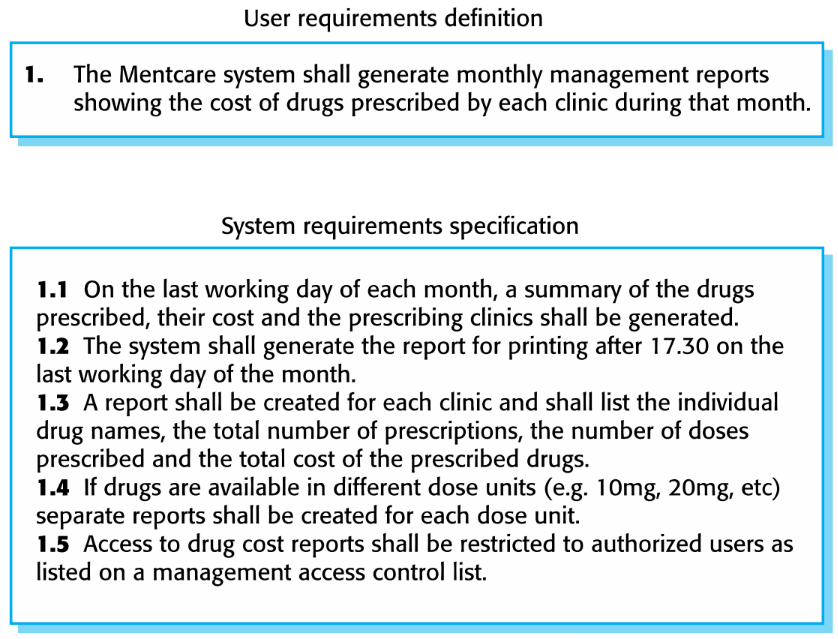
\includegraphics[width=0.6\textwidth]{images/user-system-requirements.PNG}
    %\captionof{figure}{}
\end{minipage}

È necessario scrivere i requisiti a diversi livelli di dettaglio perché tipi diversi di lettori li utilizzano in modi diversi.

\begin{minipage}{\textwidth}
    \centering
    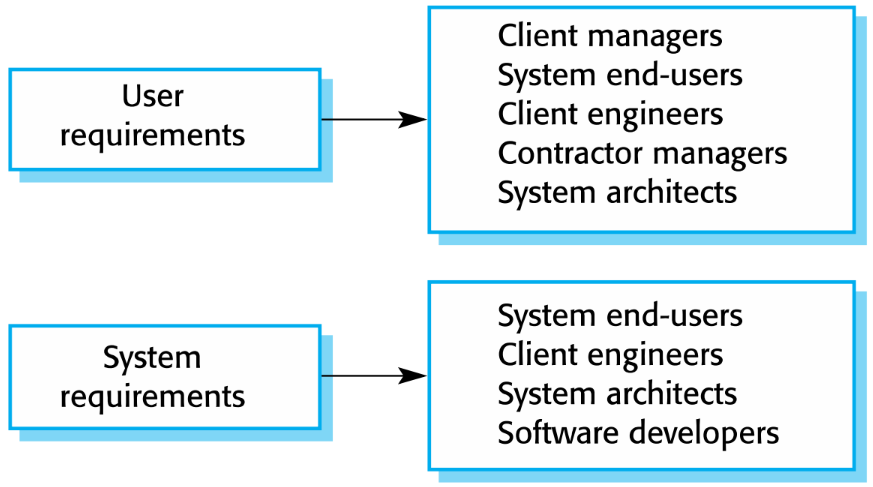
\includegraphics[width=0.5\textwidth]{images/readers-types-requirements.PNG}
    %\captionof{figure}{}
\end{minipage}
\end{Example}

I diversi tipi di lettori del documento sono esempi di stakeholder del sistema. Gli stakeholder del sistema includono chiunque sia influenzato dal sistema in qualche modo, e quindi chiunque abbia un legittimo interesse per esso. Gli stakeholder spaziano dagli utenti finali di un sistema ai manager, fino agli stakeholder esterni come i regolatori, che certificano l'accettabilità del sistema. Ad esempio, gli stakeholder del sistema Mentcare includono:
\begin{enumerate}
    \item I pazienti le cui informazioni sono registrate nel sistema e i loro parenti.
    \item I medici responsabili della valutazione e del trattamento dei pazienti.
    \item Gli infermieri che coordinano le consultazioni con i medici e somministrano alcuni trattamenti.
    \item I receptionist medici che gestiscono gli appuntamenti dei pazienti.
    \item Il personale IT che si occupa dell'installazione e della manutenzione del sistema.
    \item Un manager dell'etica medica che deve garantire che il sistema rispetti le linee guida etiche attuali per la cura dei pazienti.
    \item I manager della sanità che ottengono informazioni gestionali dal sistema.
    \item Il personale addetto ai registri medici, responsabile di garantire che le informazioni del sistema siano mantenute e conservate correttamente e che le procedure di registrazione siano state implementate.
\end{enumerate}
Molti metodi agili sostengono che produrre requisiti di sistema dettagliati sia una perdita di tempo poiché i requisiti cambiano rapidamente. I metodi agili solitamente utilizzano l'ingegneria dei requisiti incrementale e possono esprimere i requisiti come "user story". Ciò è pratico per i sistemi aziendali ma problematico per i sistemi che richiedono un'analisi pre-consegna (ad esempio, sistemi critici) o sistemi sviluppati da più team.

\section{Requisiti funzionali e non funzionali}
I requisiti di un sistema software sono spesso classificati come requisiti funzionali o non funzionali:
\begin{enumerate}
    \item \textit{Requisiti funzionali:} Questi sono dichiarazioni sui servizi che il sistema dovrebbe fornire, su come il sistema dovrebbe reagire a determinati input e su come dovrebbe comportarsi in situazioni particolari. In alcuni casi, i requisiti funzionali possono anche indicare esplicitamente cosa il sistema non dovrebbe fare.
    \item \textit{Requisiti non funzionali:} Questi sono vincoli sui servizi o sulle funzioni offerte dal sistema. Includono vincoli temporali, vincoli sul processo di sviluppo e vincoli imposti da standard. I requisiti non funzionali si applicano spesso all'intero sistema piuttosto che a singole funzionalità o servizi del sistema.
\end{enumerate}

\subsection{Requisiti funzionali}
I requisiti funzionali per un sistema descrivono cosa il sistema dovrebbe fare. Questi requisiti dipendono dal tipo di software sviluppato, dagli utenti previsti e dall'approccio generale adottato dall'organizzazione nella scrittura dei requisiti. Quando espressi come requisiti utente, i requisiti funzionali possono essere dichiarazioni di alto livello su cosa dovrebbe fare il sistema. I requisiti funzionali del sistema espandono i requisiti utente e sono scritti per gli sviluppatori del sistema. Essi devono descrivere in dettaglio le funzioni del sistema, i loro input e output, e le eccezioni.

\begin{Example}{Requisiti funzionali Mentcare}{}
\textit{Ecco alcuni esempi di requisiti funzionali per il sistema Mentcare, utilizzato per mantenere le informazioni sui pazienti che ricevono trattamenti per problemi di salute mentale:}
\begin{enumerate}
    \item Un utente deve poter cercare le liste degli appuntamenti per tutte le cliniche.
    \item Il sistema deve generare ogni giorno, per ogni clinica, una lista dei pazienti che si prevede frequentino gli appuntamenti in quel giorno.
    \item Ogni membro del personale che utilizza il sistema deve essere identificato univocamente dal suo numero dipendente a otto cifre.
\end{enumerate}
\end{Example}

L'imprecisione nella specifica dei requisiti può portare a dispute tra clienti e sviluppatori software. È naturale che uno sviluppatore interpreti un requisito ambiguo in modo tale da semplificare la sua implementazione.

Ad esempio, il primo requisito del sistema Mentcare nella lista sopra afferma che un utente deve poter cercare le liste degli appuntamenti per tutte le cliniche. La ragione di questo requisito è che i pazienti con problemi di salute mentale a volte si confondono. Potrebbero avere un appuntamento in una clinica ma in realtà recarsi in un'altra. Un membro del personale medico che specifica un requisito di ricerca potrebbe aspettarsi che "ricerca" significhi che, dato un nome di paziente, il sistema cerchi quel nome in tutti gli appuntamenti di tutte le cliniche. Tuttavia, questo non è esplicitato nel requisito. Gli sviluppatori di sistema potrebbero interpretare il requisito in modo che sia più facile da implementare. La loro funzione di ricerca potrebbe richiedere all'utente di scegliere una clinica e poi eseguire la ricerca dei pazienti che hanno frequentato quella clinica.

Idealmente, la specifica dei requisiti funzionali di un sistema dovrebbe essere completa e coerente. Completezza significa che tutti i servizi e le informazioni richiesti dall'utente dovrebbero essere definiti. Coerenza significa che i requisiti non dovrebbero essere contraddittori.

In pratica, è possibile ottenere la coerenza e la completezza dei requisiti solo per sistemi software molto piccoli.

\subsection{Requisiti non funzionali}
I requisiti non funzionali, come suggerisce il nome, sono requisiti che non riguardano direttamente i servizi specifici forniti dal sistema ai suoi utenti. Di solito, questi requisiti non funzionali specificano o vincolano le caratteristiche del sistema nel suo complesso. Possono riguardare proprietà emergenti del sistema, come l'affidabilità, il tempo di risposta e l'uso della memoria. In alternativa, possono definire vincoli sull'implementazione del sistema, come le capacità dei dispositivi di input/output o le rappresentazioni dei dati utilizzate nelle interfacce con altri sistemi.

I requisiti non funzionali sono spesso più critici dei singoli requisiti funzionali. Gli utenti del sistema possono solitamente trovare modi per aggirare una funzione del sistema che non soddisfa completamente le loro esigenze. Tuttavia, non soddisfare un requisito non funzionale può significare che l'intero sistema è inutilizzabile.

L'implementazione di questi requisiti può essere distribuita in tutto il sistema, per due motivi:
\begin{enumerate}
    \item I requisiti non funzionali possono influenzare l'architettura complessiva di un sistema piuttosto che i singoli componenti. Ad esempio, per garantire che i requisiti di prestazione siano soddisfatti in un sistema embedded, potrebbe essere necessario organizzare il sistema per minimizzare le comunicazioni tra i componenti.
    \item Un singolo requisito non funzionale, come un requisito di sicurezza, può generare diversi requisiti funzionali correlati che definiscono nuovi servizi di sistema necessari per implementare il requisito non funzionale. Inoltre, può generare requisiti che vincolano quelli esistenti; ad esempio, potrebbe limitare l'accesso alle informazioni nel sistema.
\end{enumerate}
La figura \ref{fig:types-nonfunctional-requirements} rappresenta una classificazione dei requisiti non funzionali. Da questo diagramma, si può vedere che i requisiti non funzionali possono derivare da:

\begin{figure}[ht]
    \centering
    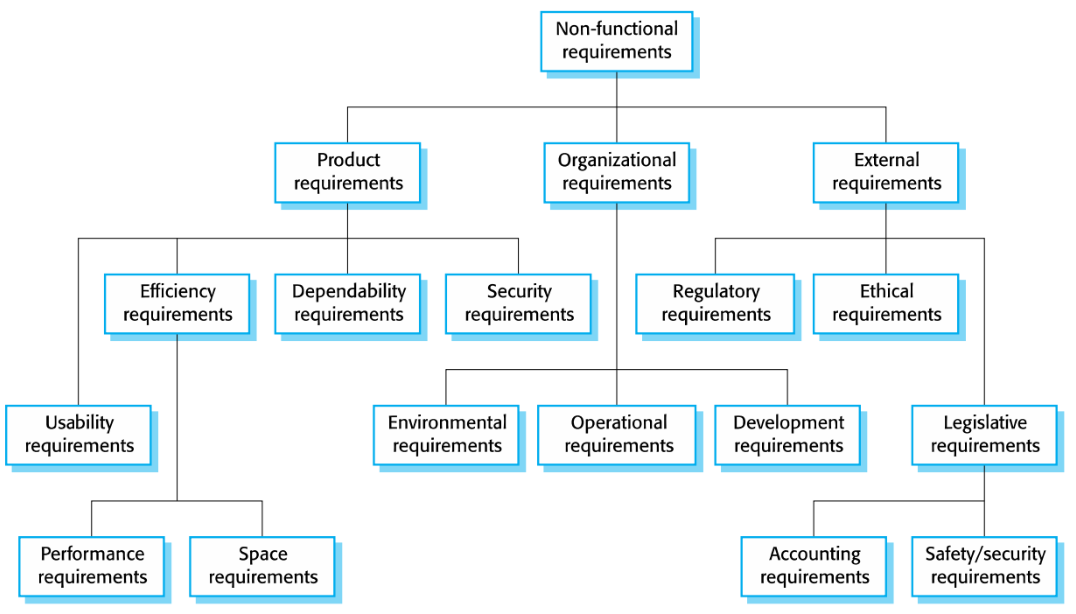
\includegraphics[width=0.7\linewidth]{images/types-nonfunctional-requirements.PNG}
    \caption{Tipi di requisiti non funzionali}
    \label{fig:types-nonfunctional-requirements}
\end{figure}

\begin{enumerate}
    \item \textit{Requisiti di prodotto:} questi requisiti specificano che il prodotto consegnato deve comportarsi in un modo particolare. Esempi includono requisiti di prestazione per la velocità di esecuzione del sistema e la quantità di memoria richiesta.
    \item \textit{Requisiti organizzativi:} questi requisiti sono conseguenza di politiche e procedure organizzative. Esempi includono requisiti del processo operativo, requisiti del processo di sviluppo o gli standard di processo da utilizzare.
    \item \textit{Requisiti esterni:} requisiti derivati da fattori esterni al sistema e al suo processo di sviluppo. Questi possono includere requisiti normativi, requisiti legislativi e requisiti etici.
\end{enumerate}

\begin{Example}{Requisiti di prodotto, organizzativi ed esterni Mentcare}{}
\textit{Vengono mostrati esempi di requisiti di prodotto, organizzativi ed esterni che potrebbero essere inclusi nella specifica del sistema Mentcare.}

\begin{enumerate}
    \item Requisito di prodotto. 
    \begin{center}
        \begin{minipage}{0.9\textwidth}
        \textit{Il sistema Mentcare deve essere disponibile per tutte le cliniche durante l'orario di lavoro normale (lun–ven, 08:30–17:30). Il tempo di inattività durante l'orario di lavoro normale non deve superare i cinque secondi in un giorno.}
    \end{minipage}
    \end{center}
    \item Requisito organizzativo.
    \begin{center}
        \begin{minipage}{0.9\textwidth}
        \textit{Gli utenti del sistema Mentcare devono autenticarsi utilizzando la loro carta d'identità dell'autorità sanitaria.}
    \end{minipage}
    \end{center}
    \item Requisito esterno.
    \begin{center}
        \begin{minipage}{0.9\textwidth}
        \textit{Il sistema deve implementare le disposizioni sulla privacy dei pazienti come stabilito in HStan-03-2006-priv.}
    \end{minipage}
    \end{center}
\end{enumerate}

Il requisito di prodotto è un requisito di disponibilità che definisce quando il sistema deve essere disponibile e il tempo di inattività consentito ogni giorno. Il requisito organizzativo specifica come gli utenti si autenticano al sistema. Il requisito esterno deriva dalla necessità che il sistema sia conforme alla legislazione sulla privacy.
\end{Example}

Un problema comune con i requisiti non funzionali è che gli stakeholder propongono requisiti come obiettivi generali, come la facilità d'uso, la capacità del sistema di recuperare da un guasto o una rapida risposta dell'utente. Gli obiettivi esprimono buone intenzioni ma causano problemi agli sviluppatori di sistema poiché lasciano spazio a interpretazioni. Ad esempio, il seguente obiettivo di sistema è tipico di come un manager potrebbe esprimere i requisiti di usabilità:
\begin{center}
    \begin{minipage}{0.9\textwidth}
    \textit{"Il sistema dovrebbe essere facile da usare per il personale medico e dovrebbe essere organizzato in modo tale da ridurre al minimo gli errori dell'utente."}
    \end{minipage}
\end{center}
È impossibile verificare oggettivamente l'obiettivo del sistema, ma nella seguente descrizione si può almeno includere la strumentazione software per contare gli errori commessi dagli utenti durante i test del sistema:
\begin{center}
    \begin{minipage}{0.9\textwidth}
    \textit{"Il personale medico deve essere in grado di utilizzare tutte le funzioni del sistema dopo due ore di formazione. Dopo questa formazione, il numero medio di errori commessi dagli utenti esperti non deve superare i due all'ora di utilizzo del sistema."}
   \end{minipage}
\end{center}
Ogni volta che possibile, i requisiti non funzionali dovrebbero essere scritti in modo quantitativo in modo che possano essere oggettivamente testati.

\begin{table}[ht]
\centering
\rowcolors{2}{lightblue}{lightgray}
\begin{tabular}{|p{4cm}|p{11cm}|}
\hline
\rowcolor{headerblue}
\textbf{\textcolor{white}{Proprietà}} & \textbf{\textcolor{white}{Misura}} \\\hline
Velocità & Transazioni elaborate al secondo \newline Tempo di risposta utente/evento \newline Tempo di aggiornamento dello schermo\\\hline
Dimensione & Megabyte \newline Numero di chip ROM\\\hline
Facilità d'uso & Tempo di formazione \newline Numero di schermate di aiuto\\\hline
Affidabilità & Tempo medio tra i guasti \newline Probabilità di indisponibilità	 \newline Tasso di occorrenza dei guasti \newline Disponibilità\\\hline
Robustezza & Tempo di riavvio dopo un guasto \newline Percentuale di eventi che causano guasti \newline Probabilità di corruzione dei dati in caso di guasto\\\hline
Portabilità & Percentuale di istruzioni dipendenti dal sistema target \newline Numero di sistemi target
\\\hline
\end{tabular}
\caption{Metriche per specificare requisiti non funzionali}
\label{tab:metrics-nonfuncional-requirements}
\end{table}

\section{Processi di ingegneria dei requisiti}
Come già discusso, l'ingegneria dei requisiti comporta tre attività chiave. Queste sono: scoprire i requisiti interagendo con gli stakeholders (elicitazione e analisi); convertire questi requisiti in una forma standard (specifica); e verificare che i requisiti definiscano effettivamente il sistema desiderato dal cliente (validazione). Nella pratica, l'ingegneria dei requisiti è un processo iterativo in cui le attività sono interconnesse. La Figura \ref{fig:spiral-requirements-engineering} mostra questa interconnessione.

\begin{figure}[ht]
    \centering
    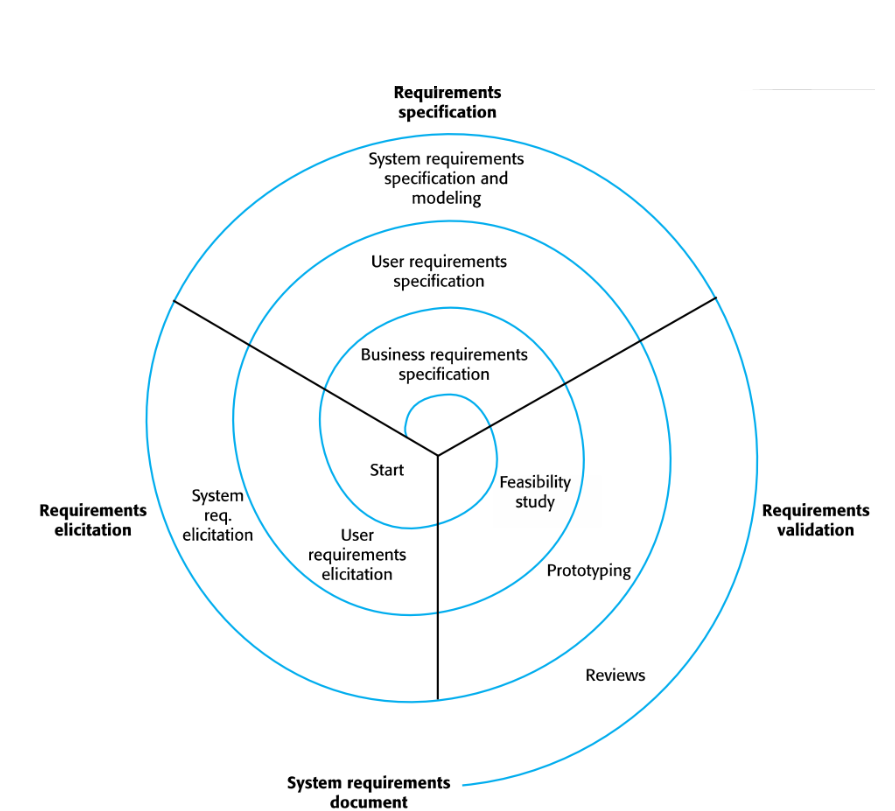
\includegraphics[width=0.7\linewidth]{images/spiral-requirements-engineering.PNG}
    \caption{Una visione a spirale del processo di ingegneria dei requisiti}
    \label{fig:spiral-requirements-engineering}
\end{figure}

\section{Elicitazione dei requisiti}
Durante l'elicitazione dei requisiti, gli ingegneri del software collaborano con gli stakeholders per ottenere informazioni sul dominio dell'applicazione, le attività lavorative, i servizi e le funzionalità del sistema richieste, le prestazioni attese dal sistema, i vincoli hardware e così via.

Elicitare e comprendere i requisiti degli stakeholders del sistema è un processo difficile per diverse ragioni:
\begin{enumerate}
    \item \textit{Difficoltà nell'esprimere i requisiti:} Gli stakeholders spesso non sanno esattamente cosa vogliono da un sistema informatico, se non in termini generali.
    \item \textit{Comprensione dei requisiti:} Gli ingegneri dei requisiti potrebbero non comprendere pienamente i requisiti del cliente, il che può portare a incomprensioni.
    \item \textit{Diversità dei requisiti:} Diversi stakeholder, con esigenze diverse, potrebbero esprimere i loro requisiti in modi differenti.
    \item \textit{Fattori politici:} I fattori politici possono influenzare i requisiti del sistema.
    \item \textit{Ambiente dinamico:} L'ambiente economico e aziendale in cui si svolge l'analisi è dinamico e cambia inevitabilmente durante il processo. Questo può portare a modifiche nei requisiti prioritari e all'emergere di nuovi requisiti da stakeholder.
\end{enumerate}
Un modello di processo dell'elicitazione e dell'analisi dei requisiti è mostrato nella Figura \ref{fig:requirements-elicitation}.

\begin{figure}[ht]
    \centering
    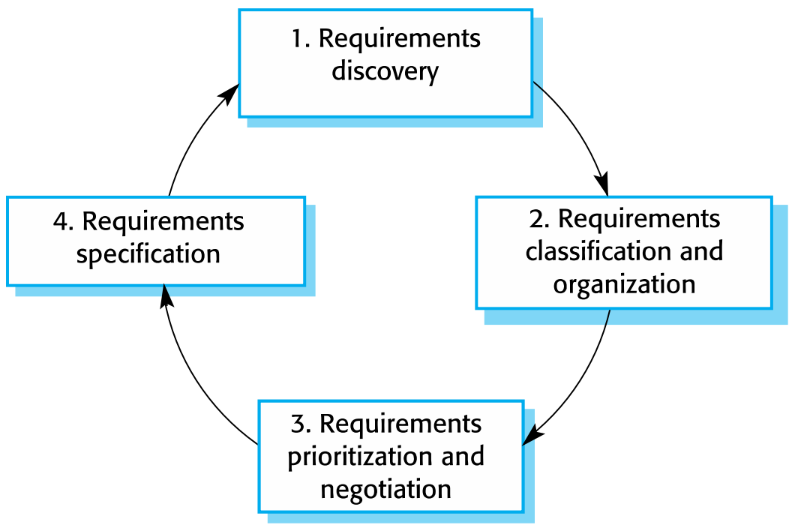
\includegraphics[width=0.5\linewidth]{images/requirements-elicitation.PNG}
    \caption{Il processo di individuazione e analisi dei requisiti}
    \label{fig:requirements-elicitation}
\end{figure}

Le attività principali del processo sono:
\begin{enumerate}
    \item \textit{Scoperta e comprensione dei requisiti:} Questo è il processo di interazione con gli stakeholders del sistema per scoprire i loro requisiti. Durante questa attività vengono scoperti anche i requisiti del dominio provenienti degli stakeholders e dalla documentazione.
    \item \textit{Classificazione e organizzazione dei requisiti:} Questa attività prende la raccolta non strutturata dei requisiti, raggruppa i requisiti correlati e li organizza in cluster coerenti.
    \item \textit{Prioritizzazione e negoziazione dei requisiti:} Questa attività si occupa di dare priorità ai requisiti e risolvere i conflitti attraverso la negoziazione.
    \item \textit{Documentazione dei requisiti:} I requisiti vengono documentati e inseriti nel ciclo successivo della spirale.
\end{enumerate}

\subsection{Tecniche di elicitazione dei requisiti}
Esistono due approcci fondamentali per l'elicitazione dei requisiti:
\begin{enumerate}
    \item Interviste, in cui si parla con le persone di ciò che fanno.
    \item Osservazione o etnografia, in cui si osservano le persone mentre svolgono il loro lavoro per vedere quali strumenti utilizzano, come li utilizzano e così via.
\end{enumerate}
È consigliabile utilizzare una combinazione di interviste e osservazione per raccogliere informazioni da cui derivare i requisiti.

\subsubsection{Interviste}
Interviste formali o informali con gli stakeholder del sistema fanno parte della maggior parte dei processi di ingegneria dei requisiti. Le interviste possono essere di due tipi:
\begin{enumerate}
    \item Interviste chiuse, in cui lo stakeholder risponde a una serie di domande predefinite.
    \item Interviste aperte, in cui vengono esplorate varie questioni con gli stakeholder.
\end{enumerate}
In pratica, le interviste con gli stakeholder sono normalmente una combinazione di entrambe queste tipologie. Potrebbe essere necessario ottenere risposte a determinate domande, ma queste di solito portano a ulteriori questioni che vengono discusse in modo meno strutturato. 

Le interviste sono utili per ottenere una comprensione generale di ciò che fanno gli stakeholder, di come potrebbero interagire con il nuovo sistema e delle difficoltà che incontrano con i sistemi attuali. Tuttavia, a meno che non si abbia un prototipo di sistema da mostrare, non bisogna aspettarsi che gli stakeholder suggeriscano requisiti specifici e dettagliati. È difficile per tutti visualizzare come potrebbe essere un sistema. È necessario analizzare le informazioni raccolte e generare i requisiti da queste.

Per essere un intervistatore efficace, è necessario tenere a mente due cose:
\begin{enumerate}
    \item Dovresti essere mentalmente aperto, evitare idee preconcette sui requisiti ed essere disposto ad ascoltare gli stakeholder.
    \item Dovresti stimolare l'intervistato per avviare le discussioni utilizzando una domanda di avvio o una proposta di requisiti, o lavorando insieme su un prototipo di sistema.
\end{enumerate}
L'elicitazione delle conoscenze del dominio attraverso le interviste può essere difficile per due motivi:
\begin{enumerate}
    \item Tutti gli specialisti di applicazioni usano un gergo specifico per il loro ambito lavorativo che gli ingegneri dei requisiti potrebbero fraintendere.
    \item Alcune conoscenze del dominio sono così familiari agli stakeholder che trovano difficile spiegarle o pensano che siano così fondamentali da non valere la pena menzionarle.
\end{enumerate}

\subsubsection{Etnografia}
L'etnografia è una tecnica di osservazione che può essere utilizzata per comprendere i processi operativi e aiutare a derivare i requisiti per il software che dovrà supportare questi processi. Un analista si immerge nell'ambiente di lavoro in cui il sistema verrà utilizzato. Si osserva il lavoro quotidiano e si prendono appunti sui compiti effettivi in cui sono coinvolti i partecipanti. Il valore dell'etnografia risiede nel fatto che aiuta a scoprire requisiti impliciti del sistema che riflettono i modi effettivi in cui le persone lavorano, piuttosto che i processi formali definiti dall'organizzazione.

L'etnografia è particolarmente efficace per scoprire due tipi di requisiti:
\begin{enumerate}
    \item Requisiti derivati dal modo in cui le persone lavorano realmente, piuttosto che dal modo in cui le definizioni dei processi aziendali dicono che dovrebbero lavorare.
    \item Requisiti derivati dalla cooperazione e dalla consapevolezza delle attività altrui. La consapevolezza di ciò che fanno le altre persone porta a cambiamenti nei modi in cui facciamo le cose.
\end{enumerate}
L'etnografia è efficace per comprendere i processi esistenti ma non può identificare nuove caratteristiche che dovrebbero essere aggiunte a un sistema.

L'etnografia può essere combinata con lo sviluppo di un prototipo di sistema (Figura \ref{fig:ethnography-prototyping-requirements}). 
\begin{figure}[ht]
    \centering
    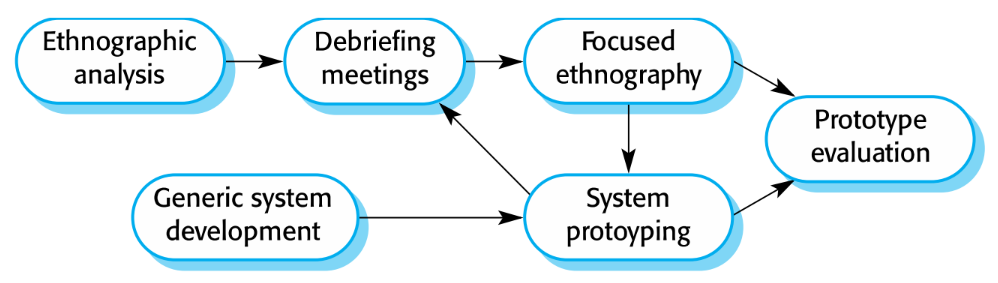
\includegraphics[width=0.6\linewidth]{images/ethnography-prototyping-requirements.PNG}
    \caption{Etnografia e prototipazione per l'analisi dei requisiti}
    \label{fig:ethnography-prototyping-requirements}
\end{figure}

\subsection{Storie e scenari}
Gli scenari e le storie degli utenti sono esempi concreti di come un sistema può essere utilizzato. Le persone trovano più facile relazionarsi a esempi di vita reale rispetto a descrizioni astratte. Storie e scenari sono modi per catturare questo tipo di informazioni. Storie e scenari sono essenzialmente la stessa cosa: una descrizione di come il sistema possa essere utilizzato per svolgere un determinato compito.

\begin{Example}{Storie e scenari iLearn}{}
\textit{Questa storia descrive una situazione in una scuola primaria (elementare) in cui l'insegnante utilizza l'ambiente per supportare progetti degli studenti sull'industria della pesca.}

Jack è un insegnante di scuola primaria a Ullapool (un villaggio nel nord della Scozia). Ha deciso che un progetto di classe sarà incentrato sull’industria della pesca nella zona, analizzando la storia, lo sviluppo e l’impatto economico della pesca. Come parte di questo, agli alunni viene chiesto di raccogliere e condividere ricordi di parenti, usare archivi di giornali e collezionare vecchie fotografie legate alla pesca e alle comunità di pescatori della zona. Gli alunni usano un wiki di iLearn per raccogliere storie sulla pesca e SCRAN (un sito di risorse storiche) per accedere agli archivi di giornali e fotografie. Tuttavia, Jack ha anche bisogno di un sito per condividere foto, poiché vuole che gli alunni possano scattare foto, commentarle reciprocamente e caricare scansioni di vecchie fotografie che potrebbero avere in famiglia.

Jack invia un’email a un gruppo di insegnanti di scuola primaria, di cui è membro, per vedere se qualcuno può consigliargli un sistema adatto. Due insegnanti rispondono e entrambi suggeriscono di utilizzare KidsTakePics, un sito di condivisione di foto che consente agli insegnanti di controllare e moderare i contenuti. Poiché KidsTakePics non è integrato con il servizio di autenticazione di iLearn, Jack crea un account per sé e uno per la classe. Usa il servizio di configurazione di iLearn per aggiungere KidsTakePics ai servizi visualizzati dagli alunni della sua classe, in modo che, quando si collegano, possano utilizzare immediatamente il sistema per caricare foto dai loro dispositivi mobili e dai computer della classe.
\begin{itemize}
    \item \textit{Ipotesi iniziale:} Un utente o un gruppo di utenti ha una o più fotografie digitali da caricare sul sito di condivisione foto. Queste sono salvate su un tablet o su un computer portatile. Gli utenti si sono collegati con successo a KidsTakePics.

    \item \textit{Normale:} L’utente sceglie l’opzione per caricare le foto e viene invitato a selezionare le foto da caricare sul proprio computer e a scegliere il nome del progetto sotto il quale verranno archiviate le foto. Gli dovrebbe anche essere data l’opzione di inserire parole chiave associate a ciascuna foto caricata. Le foto caricate vengono nominate creando una combinazione del nome utente e del nome del file della foto sul computer locale.
    
    Al termine del caricamento, il sistema invia automaticamente un’email al moderatore del progetto per chiedergli di controllare il nuovo contenuto e genera un messaggio sullo schermo per l’utente, informandolo che il caricamento è stato completato.

    \item \textit{Cosa può andare storto:} Nessun moderatore è associato al progetto selezionato. Viene automaticamente generata un’email per l’amministratore della scuola chiedendogli di nominare un moderatore di progetto. Agli utenti dovrebbe essere comunicato che potrebbe esserci un ritardo nel rendere visibili le loro foto.

    Foto con lo stesso nome sono già state caricate dallo stesso utente. All’utente dovrebbe essere chiesto se desidera ricaricare le foto con lo stesso nome, rinominare le foto o annullare il caricamento. Se sceglie di ricaricare le foto, le originali vengono sovrascritte. Se sceglie di rinominare le foto, viene generato automaticamente un nuovo nome aggiungendo un numero al nome del file esistente.

    \item \textit{Altre attività:} Il moderatore potrebbe essere collegato al sistema e approvare le foto man mano che vengono caricate.

    \item \textit{Stato del sistema al termine:} L’utente è collegato. Le foto selezionate sono state caricate e assegnate con lo stato “in attesa di moderazione”. Le foto sono visibili al moderatore e all’utente che le ha caricate.
\end{itemize}
\end{Example}

A livello generale, uno scenario può includere:
\begin{enumerate}
    \item Una descrizione di cosa si aspetta il sistema e gli utenti quando inizia lo scenario.
    \item Una descrizione del flusso normale degli eventi nello scenario.
    \item Una descrizione di ciò che può andare storto e di come gestire i problemi che ne derivano.
    \item Informazioni su altre attività che potrebbero essere in corso contemporaneamente.
    \item Una descrizione dello stato del sistema al termine dello scenario.
\end{enumerate}

\section{Specifica dei requisiti}
La specifica dei requisiti è il processo di scrittura dei requisiti utente e dei requisiti di sistema in un documento di requisiti. Idealmente, i requisiti utente e di sistema dovrebbero essere chiari, univoci, facili da comprendere, completi e coerenti. I requisiti utente devono essere comprensibili per gli utenti finali e i clienti che non hanno una formazione tecnica. I requisiti di sistema sono requisiti più dettagliati e possono includere più informazioni tecniche. I requisiti possono essere parte di un contratto per lo sviluppo del sistema, è quindi importante che siano il più completi possibile.

\begin{table}[ht]
\centering
\rowcolors{2}{lightblue}{lightgray}
\begin{tabular}{|p{4cm}|p{11cm}|}
\hline
\rowcolor{headerblue}
\textbf{\textcolor{white}{Notazione}} & \textbf{\textcolor{white}{Descrizione}} \\\hline
Linguaggio naturale & I requisiti sono scritti usando frasi numerate in linguaggio naturale. Ogni frase dovrebbe esprimere un requisito.\\\hline
Linguaggio naturale strutturato & I requisiti sono scritti in linguaggio naturale su un modulo o modello standard. Ogni campo fornisce informazioni su un aspetto del requisito.\\\hline
Linguaggi di descrizione del design & Questo approccio utilizza un linguaggio simile a un linguaggio di programmazione, ma con caratteristiche più astratte per specificare i requisiti definendo un modello operativo del sistema. Questo metodo è ora raramente usato, ma può essere utile per le specifiche delle interfacce.\\\hline
Notazioni grafiche & Modelli grafici, integrati da annotazioni testuali, vengono utilizzati per definire i requisiti funzionali del sistema; i diagrammi dei casi d'uso e di sequenza UML sono comunemente utilizzati.\\\hline
Specifiche matematiche & Queste notazioni si basano su concetti matematici come macchine a stati finiti o insiemi. Sebbene queste specifiche prive di ambiguità possano ridurre l'ambiguità in un documento di requisiti, la maggior parte dei clienti non comprende una specifica formale. Non possono verificare che essa rappresenti ciò che desiderano e sono riluttanti ad accettarla come contratto per il sistema.
\\\hline
\end{tabular}
\caption{Modi di scrivere una specifica dei requisiti di sistema}
\label{tab:writing-system-requirements}
\end{table}

Idealmente, i requisiti di sistema dovrebbero descrivere solo il comportamento esterno del sistema e i suoi vincoli operativi, senza riguardare il modo in cui il sistema dovrebbe essere progettato o implementato. Tuttavia, nella pratica, i requisiti e la progettazione sono inseparabili:
\begin{enumerate}
    \item Potrebbe essere necessario progettare un'architettura iniziale del sistema per aiutare a strutturare la specifica dei requisiti.
    \item Nella maggior parte dei casi, i sistemi devono interoperare con sistemi esistenti, il che vincola la progettazione e impone requisiti sul nuovo sistema.
    \item L'uso di una specifica architettura per soddisfare requisiti non funzionali potrebbe essere necessario. Un regolatore esterno che deve certificare la sicurezza del sistema potrebbe specificare che venga utilizzato un design architettonico già certificato.
\end{enumerate}

\subsection{Specifica in linguaggio naturale}
I requisiti sono scritti come frasi in linguaggio naturale integrate da diagrammi e tabelle. È espressivo, intuitivo e universale. Ciò significa che i requisiti possono essere compresi da utenti e clienti. Per ridurre i malintesi quando si scrivono requisiti in linguaggio naturale, raccomando di seguire queste semplici linee guida:
\begin{enumerate}
    \item Creare un formato standard e assicurarsi che tutte le definizioni dei requisiti aderiscano a tale formato.
    \item Utilizzare un linguaggio coerente per distinguere tra requisiti obbligatori e desiderabili. 
    \item Utilizzare l’evidenziazione del testo (grassetto, corsivo o colore) per mettere in risalto le parti chiave del requisito.
    \item Non presumere che i lettori comprendano il linguaggio tecnico o di ingegneria del software. Evitare, dove possibile, l'uso di gergo, abbreviazioni e acronimi.
    \item Includere una spiegazione (motivazione) del perché un requisito è necessario.
\end{enumerate}
I problemi che possono sorgere utilizzando il linguaggio naturale per i requisiti sono:
\begin{enumerate}
    \item \textit{Mancanza di chiarezza:} La precisione è difficile senza rendere il documento difficile da leggere. 
    \item \textit{Confusione dei requisiti:} I requisiti funzionali e non funzionali tendono a essere confusi. 
    \item \textit{Fusione dei requisiti:} Possono essere espressi insieme diversi requisiti.
\end{enumerate}

\begin{Example}{Requisiti per la pompa per insulina}{}
\textit{Vengono mostrate come applicare le linee guida, includendo due requisiti per il software incorporato nella pompa per insulina automatizzata.}    
\begin{enumerate}
    \item Il sistema deve misurare la glicemia e somministrare insulina, se necessario, ogni 10 minuti. (Le variazioni della glicemia sono relativamente lente, quindi una misurazione più frequente non è necessaria; una misurazione meno frequente potrebbe portare a livelli di zucchero inutilmente alti.)
    \item Il sistema deve eseguire una routine di autotest ogni minuto, con le condizioni da testare e le azioni associate definite. (Una routine di autotest può individuare problemi hardware e software e avvisare l’utente del fatto che il normale funzionamento potrebbe non essere possibile.)
\end{enumerate}
\end{Example}

\subsection{Specifiche strutturate}
Le specifiche strutturate in linguaggio naturale rappresentano un metodo per scrivere i requisiti di sistema utilizzando un formato standard, anziché un testo libero.

%Un esempio di specifica basata su moduli, in questo caso per il calcolo della dose di insulina da somministrare quando il livello di zucchero nel sangue rientra in un intervallo sicuro, è mostrato nella Figura 4.13.

Quando si utilizza un formato standard per specificare i requisiti funzionali, dovrebbero essere incluse le seguenti informazioni:
\begin{enumerate}
    \item Descrizione della funzione o entità specificata.
    \item Descrizione degli input e della loro origine.
    \item Descrizione degli output e della loro destinazione.
    \item Informazioni sui dati necessari per il calcolo o altre entità richieste nel sistema.
    \item Descrizione dell'azione da eseguire.
    \item Se si utilizza un approccio funzionale, una precondizione che indica ciò che deve essere vero prima che la funzione sia chiamata, e una postcondizione che indica ciò che è vero dopo che la funzione è stata chiamata.
    \item Descrizione degli effetti collaterali (se presenti) dell'operazione.
\end{enumerate}
Tuttavia, può comunque risultare difficile scrivere requisiti in modo chiaro e non ambiguo, specialmente quando è necessario specificare calcoli complessi (ad esempio, come calcolare la dose di insulina). Per affrontare questo problema, è possibile aggiungere informazioni extra ai requisiti in linguaggio naturale, ad esempio tramite tabelle o modelli grafici del sistema. Le tabelle sono particolarmente utili quando ci sono diverse situazioni alternative e si devono descrivere le azioni da intraprendere per ciascuna di esse. 

\begin{Example}{Specifica strutturata per la pompa per insulina}{}
\texttt{Insulin Pump/Control Software/SRS/3.3.2}
\begin{itemize}
    \item \textit{Funzione:} Calcolo della dose di insulina: livello sicuro di zucchero.
    \item \textit{Descrizione:} Calcola la dose di insulina da somministrare quando il livello di zucchero attuale misurato rientra nella zona sicura tra 3 e 7 unità.
    \item \textit{Input:} Lettura attuale del livello di zucchero ($r_2$); le due letture precedenti ($r_0$ e $r_1$).
    \item \textit{Fonte:} Lettura attuale del livello di zucchero dal sensore. Altre letture dalla memoria.
    \item \textit{Output:} \texttt{CompDose} - la dose di insulina da somministrare.
    \item \textit{Destinazione:} Ciclo di controllo principale.
    \item \textit{Azione:} \texttt{CompDose} è zero se il livello di zucchero è stabile o in diminuzione, oppure se il livello è in aumento ma il tasso di aumento è in diminuzione. Se il livello è in aumento e il tasso di aumento sta aumentando, allora \texttt{CompDose} è calcolato dividendo la differenza tra il livello di zucchero attuale e quello precedente per 4 e arrotondando il risultato. Se il risultato è arrotondato a zero, \texttt{CompDose} viene impostato alla dose minima che può essere somministrata.
    \item \textit{Requisiti:} Due letture precedenti per calcolare il tasso di variazione del livello di zucchero.
    \item \textit{Pre-condizione:} Il serbatoio di insulina contiene almeno la dose singola massima consentita di insulina.
    \item \textit{Post-condizione:} $r_0$ viene sostituito da $r_1$, quindi $r_1$ viene sostituito da $r_2$.
    \item \textit{Effetti collaterali:} Nessuno.
\end{itemize}

La pompa per insulina basa i suoi calcoli del fabbisogno di insulina sul tasso di variazione dei livelli di zucchero nel sangue. Si può usare una descrizione tabellare di come il tasso di variazione dello zucchero nel sangue viene utilizzato per calcolare la quantità di insulina da somministrare.\\

\begin{minipage}{\textwidth}
\rowcolors{2}{lightblue}{lightgray}
\begin{tabular}{|p{7.5cm}|p{6cm}|}
\hline
\rowcolor{headerblue}
\textbf{\textcolor{white}{Condizione}} & \textbf{\textcolor{white}{Azione}} \\\hline
Livello di zucchero in diminuzione ($r_2 < r_1$) & $CompDose = 0$\\\hline
Livello di zucchero stabile ($r_2 = r_1$) & $CompDose = 0$\\\hline
Livello di zucchero in aumento e tasso di aumento in diminuzione ($(r_2-r_1)<(r_1-r_0)$) & $CompDose = 0$\\\hline
Livello di zucchero in aumento e tasso di aumento stabile o in aumento ($(r_2-r_1)\geq (r_1-r_0)$) & $CompDose = round((r_2-r_1)/4)$ \texttt{if rounded result=0 then} $CompDose = MinimumDose$
\\\hline
\end{tabular}
\end{minipage}
\end{Example}

\subsection{Use cases}
I casi d'uso sono un modo per descrivere le interazioni tra gli utenti e un sistema utilizzando un modello grafico e un testo strutturato. Sono diventati una caratteristica fondamentale del Linguaggio di Modellazione Unificato (UML). Nella loro forma più semplice, un caso d'uso identifica gli attori coinvolti in un'interazione e nomina il tipo di interazione. L'insieme dei casi d'uso rappresenta tutte le possibili interazioni che saranno descritte nei requisiti di sistema.

La Figura \ref{fig:use-case-mantcare}, mostra alcuni dei casi d'uso per il sistema Mentcare.

\begin{figure}[ht]
    \centering
    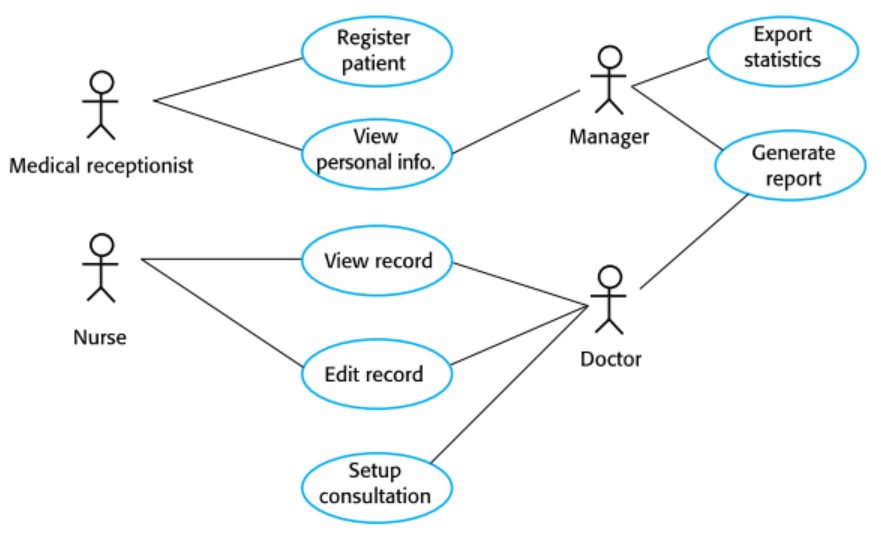
\includegraphics[width=0.6\linewidth]{images/use-case-mentcare.PNG}
    \caption{Casi d'uso per il sistema Mentcare}
    \label{fig:use-case-mantcare}
\end{figure}

\subsection{Documento sui requisiti software}
Il documento dei requisiti software (chiamato talvolta specifica dei requisiti software o SRS) è una dichiarazione ufficiale di ciò che gli sviluppatori di sistemi dovrebbero implementare. Può includere sia i requisiti degli utenti per un sistema sia una specifica dettagliata dei requisiti di sistema. Non è un documento di progettazione e, per quanto possibile, dovrebbe impostare cosa dovrebbe fare il sistema piuttosto che come dovrebbe farlo.

Il documento dei requisiti ha un insieme di utenti diversificato. La Figura \ref{fig:users-requirements-document} mostra i possibili utenti del documento e come lo utilizzano.

\begin{figure}[ht]
    \centering
    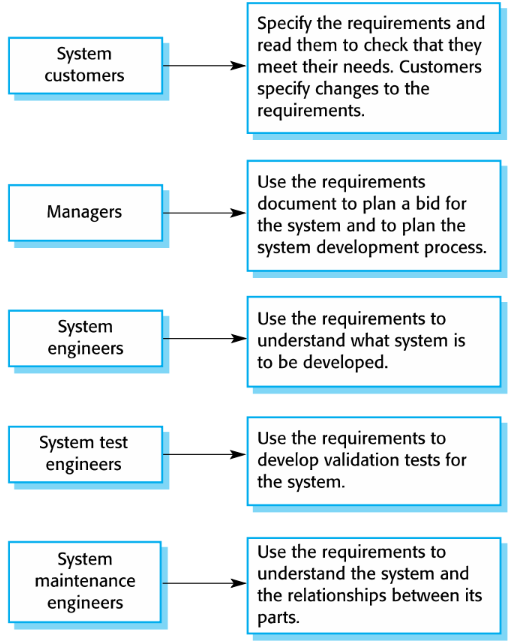
\includegraphics[width=0.5\linewidth]{images/users-requirements-document.PNG}
    \caption{Utenti di un documento di requisiti}
    \label{fig:users-requirements-document}
\end{figure}

Il livello di dettaglio da includere in un documento di requisiti dipende dal tipo di sistema che viene sviluppato e dal processo di sviluppo utilizzato. I sistemi critici necessitano di requisiti dettagliati perché la sicurezza e l'affidabilità devono essere analizzate in dettaglio per trovare possibili errori nei requisiti. Se viene utilizzato un processo di sviluppo iterativo interno, il documento dei requisiti può essere meno dettagliato. I dettagli possono essere aggiunti ai requisiti e le ambiguità risolte durante lo sviluppo del sistema.

Sono stati progettati standard per i documenti dei requisiti, ad esempio lo standard IEEE (vedi Tabella \ref{tab:structure-requirements-document}). Questi sono per lo più applicabili ai requisiti per grandi progetti di ingegneria dei sistemi.

\begin{table}[ht]
\centering
\rowcolors{2}{lightblue}{lightgray}
\begin{tabular}{|p{4cm}|p{11cm}|}
\hline
\rowcolor{headerblue}
\textbf{\textcolor{white}{Capitolo}} & \textbf{\textcolor{white}{Descrizione}} \\\hline
Prefazione & Dovrebbe definire il pubblico previsto del documento e descriverne la storia delle versioni, inclusa una motivazione per la creazione di una nuova versione e un riassunto delle modifiche apportate in ciascuna versione.\\\hline
Introduzione & Dovrebbe descrivere la necessità del sistema, riassumerne le funzioni e spiegare come funzionerà con altri sistemi. Dovrebbe inoltre descrivere come il sistema si inserisce negli obiettivi aziendali o strategici dell'organizzazione committente.\\\hline
Glossario & Dovrebbe definire i termini tecnici usati nel documento, senza presupporre esperienze o competenze del lettore.\\\hline
Definizione dei requisiti utente & Qui si descrivono i servizi forniti per l'utente. Anche i requisiti di sistema non funzionali devono essere descritti in questa sezione. La descrizione può utilizzare il linguaggio naturale, diagrammi o altre notazioni comprensibili ai clienti. Inoltre, devono essere specificati gli standard di prodotto e di processo da seguire.\\\hline
Architettura di sistema & Questo capitolo dovrebbe presentare una panoramica di alto livello dell'architettura prevista del sistema, mostrando la distribuzione delle funzioni nei moduli del sistema. I componenti architetturali riutilizzati dovrebbero essere evidenziati.\\\hline
Specifica dei requisiti di sistema & Dovrebbe descrivere in dettaglio i requisiti funzionali e non funzionali. Se necessario, ulteriori dettagli possono essere aggiunti ai requisiti non funzionali. Possono essere definite le interfacce con altri sistemi.\\\hline
Modelli di sistema & Potrebbe includere modelli grafici del sistema che mostrano le relazioni tra i componenti del sistema e tra il sistema e il suo ambiente. Esempi di modelli possibili sono modelli a oggetti, modelli di flusso di dati o modelli di dati semantici.\\\hline
Evoluzione del sistema & Dovrebbe descrivere i presupposti fondamentali su cui si basa il sistema e i cambiamenti previsti dovuti all'evoluzione dell'hardware, ai cambiamenti nelle esigenze degli utenti, ecc. Questa sezione è utile ai progettisti del sistema, poiché può aiutarli a evitare decisioni di progettazione che limiterebbero futuri cambiamenti.\\\hline
Appendici & Dovrebbero fornire informazioni dettagliate e specifiche relative all'applicazione in fase di sviluppo; ad esempio, descrizioni dell'hardware e del database. I requisiti hardware definiscono le configurazioni minime e ottimali per il sistema. I requisiti di database definiscono l'organizzazione logica dei dati utilizzati dal sistema e le relazioni tra i dati.\\\hline
Indice & Possono essere inclusi vari indici del documento. Oltre a un indice alfabetico normale, possono esserci un indice dei diagrammi, un indice delle funzioni, ecc.
\\\hline
\end{tabular}
\caption{La struttura di un documento di requisiti}
\label{tab:structure-requirements-document}
\end{table}

\section{Validazione dei requisiti}
La validazione dei requisiti è il processo di verifica che i requisiti definiscano il sistema che il cliente desidera realmente. La validazione dei requisiti è di importanza cruciale, poiché errori in un documento dei requisiti possono portare a costi di rifacimento significativi quando questi problemi vengono scoperti durante lo sviluppo o dopo che il sistema è in servizio.

Il costo per correggere un problema nei requisiti attraverso una modifica del sistema è solitamente molto maggiore rispetto alla correzione di errori di progettazione o di codifica. Una modifica dei requisiti di solito comporta anche cambiamenti nella progettazione e nell’implementazione del sistema, che devono poi essere nuovamente testati.

Durante il processo di validazione dei requisiti, devono essere eseguiti diversi tipi di controlli sui requisiti nel documento dei requisiti:
\begin{enumerate}
    \item \textit{Controlli di validità:} verificano che i requisiti riflettano le reali esigenze degli utenti del sistema.
    \item \textit{Controlli di coerenza:} i requisiti nel documento non devono essere in conflitto tra loro, ossia non devono esserci vincoli contraddittori o descrizioni differenti della stessa funzione di sistema.
    \item \textit{Controlli di completezza:} il documento dei requisiti dovrebbe includere i requisiti che definiscono tutte le funzioni e i vincoli previsti dall’utente del sistema.
    \item \textit{Controlli di realismo:} basandosi sulla conoscenza delle tecnologie esistenti, i requisiti devono essere verificati per assicurarsi che possano essere implementati entro il budget proposto per il sistema.
    \item \textit{Verificabilità:} i requisiti del sistema devono sempre essere scritti in modo che siano verificabili.
\end{enumerate}
Diverse tecniche di validazione dei requisiti possono essere utilizzate individualmente o in combinazione tra loro:
\begin{enumerate}
    \item \textit{Revisione dei requisiti:} i requisiti sono analizzati sistematicamente da un team di revisori che verifica la presenza di errori e incoerenze.
    \item \textit{Prototipazione:} consiste nello sviluppo di un modello eseguibile di un sistema e nel suo utilizzo con utenti finali e clienti per verificare se soddisfa le loro esigenze e aspettative.
    \item \textit{Generazione di casi di test:} sviluppo di test per i requisiti per verificarne la testabilità.
\end{enumerate}
Si dovrebbero tenere delle revisioni regolari mentre si formula la definizione dei requisiti. Sia il personale del cliente che quello dell'appaltatore dovrebbero essere coinvolti nelle revisioni. Le revisioni possono essere formali (con documenti completati) o informali. Una buona comunicazione tra sviluppatori, clienti e utenti può risolvere i problemi in una fase iniziale.

\section{Requisiti in continua evoluzione}
I requisiti per i grandi sistemi software cambiano sempre. La maggior parte delle modifiche ai requisiti del sistema si verifica a causa di cambiamenti nell'ambiente aziendale del sistema:
\begin{enumerate}
    \item L'ambiente aziendale e tecnico del sistema cambia sempre dopo l'installazione. Potrebbe essere introdotto nuovo hardware e l'hardware esistente aggiornato. Potrebbe essere necessario interfacciare il sistema con altri sistemi. Le priorità aziendali possono cambiare e potrebbero essere introdotte nuove leggi e normative che richiedono la conformità del sistema.
    \item Chi paga per un sistema e chi lo utilizza sono raramente le stesse persone. I clienti del sistema impongono requisiti a causa di vincoli organizzativi e di budget. Questi possono entrare in conflitto con i requisiti degli utenti finali, e, dopo la consegna, potrebbero dover essere aggiunte nuove funzionalità per supportare gli utenti affinché il sistema raggiunga i suoi obiettivi.
    \item I grandi sistemi di solito hanno una comunità di stakeholder diversificata, con stakeholder che hanno requisiti differenti. Le loro priorità possono essere in conflitto o contraddittorie. I requisiti finali del sistema sono inevitabilmente un compromesso, e alcuni stakeholder devono essere prioritizzati. Con l’esperienza, spesso si scopre che è necessario modificare l’equilibrio del supporto fornito ai diversi stakeholder e riprioritizzare i requisiti.
\end{enumerate}

\begin{figure}[ht]
    \centering
    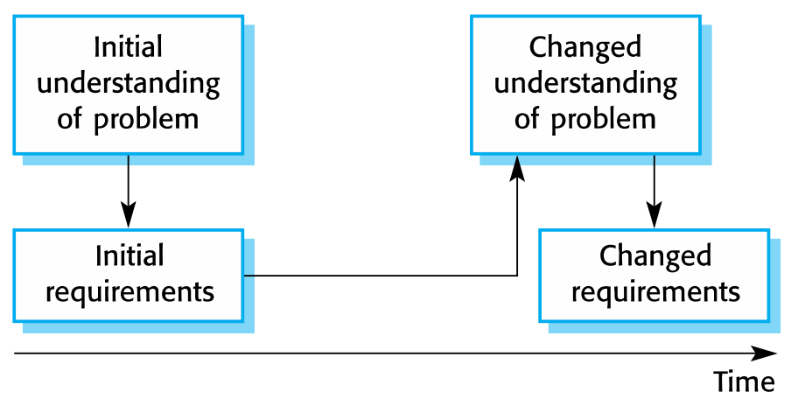
\includegraphics[width=0.4\linewidth]{images/requirements-evolution.PNG}
    \caption{Evoluzione dei requisiti}
    \label{fig:requirements-evolution}
\end{figure}

La gestione dei requisiti è il processo di gestione dei requisiti in evoluzione durante il processo di ingegneria dei requisiti e lo sviluppo del sistema. Nuovi requisiti emergono man mano che un sistema viene sviluppato e dopo che è stato messo in uso. È necessario monitorare i requisiti individuali e mantenere i collegamenti tra i requisiti dipendenti in modo da poter valutare l'impatto delle modifiche ai requisiti. È importante stabilire un processo formale per presentare proposte di modifica e collegarle ai requisiti del sistema.

\subsection{Pianificazione della gestione dei requisiti}
La pianificazione della gestione dei requisiti riguarda la definizione di come gestire un insieme di requisiti in evoluzione. Durante questa fase, è necessario prendere decisioni su vari aspetti:
\begin{enumerate}
    \item \textit{Identificazione dei requisiti:} ogni requisito deve essere identificato in modo univoco, così da poter essere collegato ad altri requisiti e utilizzato nelle valutazioni di tracciabilità.
    \item \textit{Processo di gestione delle modifiche:} si tratta di una serie di attività per valutare l'impatto e il costo delle modifiche.
    \item \textit{Politiche di tracciabilità:} queste politiche definiscono le relazioni da registrare tra ciascun requisito e tra i requisiti e il design del sistema.
    \item \textit{Supporto tramite strumenti:} gli strumenti utilizzati possono variare da sistemi specializzati per la gestione dei requisiti a fogli di calcolo condivisi e semplici database.
\end{enumerate}

\subsection{Gestione delle modifiche ai requisiti}
La gestione delle modifiche ai requisiti (Figura \ref{fig:requirements-change-management}) deve essere applicata a tutte le modifiche proposte ai requisiti di un sistema dopo l'approvazione del documento dei requisiti. 

\begin{figure}[ht]
    \centering
    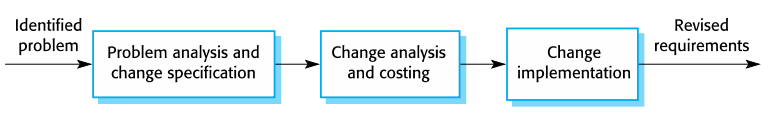
\includegraphics[width=0.7\linewidth]{images/requirements-change-management.PNG}
    \caption{Gestione dei cambiamenti dei requisiti}
    \label{fig:requirements-change-management}
\end{figure}

Esistono tre fasi principali in un processo di gestione delle modifiche:
\begin{enumerate}
    \item \textit{Analisi del problema e specifica della modifica:} in questa fase, il problema o la proposta viene analizzata per verificarne la validità. Questa analisi viene comunicata al richiedente della modifica, che può rispondere con una proposta di modifica più dettagliata o decidere di ritirare la richiesta.
    \item \textit{Analisi e stima del costo della modifica:} l'effetto della modifica proposta viene valutato utilizzando le informazioni di tracciabilità e la conoscenza generale dei requisiti del sistema. Completata questa analisi, si decide se procedere o meno con la modifica dei requisiti.
    \item \textit{Implementazione della modifica:} il documento dei requisiti e, se necessario, la progettazione e l'implementazione del sistema, vengono modificati. È opportuno organizzare il documento dei requisiti in modo che sia possibile apportare modifiche senza riscrivere o riorganizzare ampiamente il documento.
\end{enumerate}

\newpage
\section{Punti chiave}
\begin{center}
\begin{minipage}{\textwidth}
\colorbox{lightgray}{
\parbox{\linewidth}{
\begin{itemize} 
    \item I requisiti per un sistema software stabiliscono cosa il sistema dovrebbe fare e definiscono i vincoli sulla sua operatività e implementazione.
    \item I requisiti funzionali sono dichiarazioni dei servizi che il sistema deve fornire o descrizioni di come devono essere eseguiti alcuni calcoli.
    \item I requisiti non funzionali spesso vincolano il sistema in fase di sviluppo e il processo di sviluppo stesso.
    
    Essi riguardano frequentemente le proprietà emergenti del sistema e quindi si applicano al sistema nel suo insieme.
    \item Il processo di ingegneria dei requisiti è un processo iterativo che include l'elicitazione, la specifica e la validazione dei requisiti.
    \item L'elicitazione dei requisiti è un processo iterativo che può essere rappresentato come una spirale di attività: scoperta dei requisiti, classificazione e organizzazione dei requisiti, negoziazione e documentazione dei requisiti.
    \item È possibile utilizzare una varietà di tecniche per l'elicitazione dei requisiti, tra cui interviste ed etnografia. Storie utente e scenari possono essere utilizzati per facilitare le discussioni.
    \item La specifica dei requisiti è il processo di documentazione formale dei requisiti utente e di sistema e di creazione di un documento dei requisiti software.
    \item Il documento dei requisiti software è una dichiarazione concordata dei requisiti del sistema. Dovrebbe essere organizzato in modo che sia i clienti del sistema che i sviluppatori software possano utilizzarlo.
    \item La validazione dei requisiti è il processo di verifica dei requisiti per validità, coerenza, completezza, realismo e verificabilità.
    \item I cambiamenti aziendali, organizzativi e tecnici portano inevitabilmente a modifiche nei requisiti per un sistema software. La gestione dei requisiti è il processo di gestione e controllo di tali cambiamenti.
\end{itemize}
}}
\end{minipage}
\end{center}